\documentclass[border=10pt]{standalone}
\usepackage{tikz}
\usetikzlibrary{automata, positioning, arrows.meta}

\begin{document}
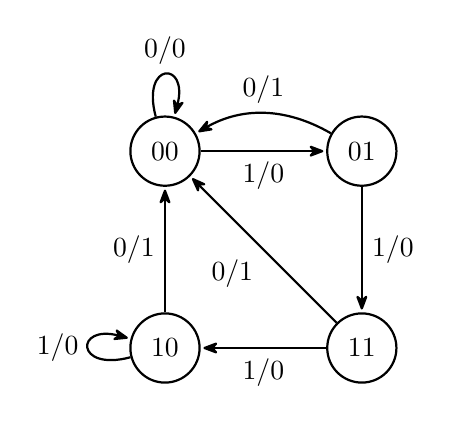
\begin{tikzpicture}[shorten >=1pt, node distance=2.5cm, on grid, auto, >={Stealth[round]}, thick]
    % Nodes
    \node[state] (s00) {00};
    \node[state] (s01) [right=of s00] {01};
    \node[state] (s10) [below=of s00] {10};
    \node[state] (s11) [below=of s01] {11};

    % Transitions based on Table:
    % 00 -> 00 (0/0), 00 -> 01 (1/0)
    % 01 -> 00 (0/1), 01 -> 11 (1/0)
    % 10 -> 00 (0/1), 10 -> 10 (1/0)
    % 11 -> 00 (0/1), 11 -> 10 (1/0)

    \path[->]
        (s00) edge [loop above] node {0/0} (s00)
              edge node [swap] {1/0} (s01)
              
        (s01) edge [bend right] node [swap] {0/1} (s00)
              edge node {1/0} (s11)
              
        (s10) edge node {0/1} (s00)
              edge [loop left] node {1/0} (s10)
              
        (s11) edge node {1/0} (s10)
              edge node {0/1} (s00);

\end{tikzpicture}
\end{document}
